\newif\ifisdraft
\isdraftfalse
\newcommand{\isdraft}{\ifisdraft true\else false\fi}
\newcommand{\todo}[1]{
  \ifisdraft {
    \Large
    $\color{black}\star$\color{red}~\textit{#1}\color{black}~$\star$
  } \fi
}

% Used in advected_subdomain.tex
\definecolor{advectionColor}{RGB}{213,94,0}   % vermillion / orange
\definecolor{diffusionColor}{RGB}{0,114,178}  % blue

\definecolor{powderColor}{rgb}{0.878,0.859,0.811}
\definecolor{metalColor}{rgb}{0.420,0.408,0.384}
\newcommand{\legendpowderbulk}{%
  \begin{tabular}{rlrl}
     ({\color{powderColor} \rule[-1.5 pt]{8 pt}{8 pt}}) & Powder & ({\color{metalColor} \rule[-1.5 pt]{8 pt}{8 pt}})  & Bulk
  \end{tabular}
}
\newcommand{\wireframeTriangle}{%
    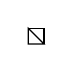
\begin{tikzpicture}[scale=0.2] % adjust scale as needed
      % Bottom triangle
      \draw[]
        (0,0) coordinate (A)
        -- (0,1) coordinate (B)
        -- (1,0) coordinate (C)
        -- cycle;
      % Upper triangle
      \draw[]
        (0,1) coordinate (D)
        -- (1,1) coordinate (E)
        -- (1,0) coordinate (F);
    \end{tikzpicture}
}

\newcommand{\playthumb}[2][]{%
  \begin{tikzpicture}
    % Thumbnail image
    \node[inner sep=0] (img) {\includegraphics[#1]{#2}};
    % Dark circle
    \draw[fill=black!60, draw=white, line width=0.8pt]
      (img.center) circle[radius=0.6cm];
    % Triangle
    \draw[fill=white, draw=none, rounded corners=1.5pt]
      ([xshift=0.34cm]img.center) --
      ([xshift=-0.19cm,yshift=0.3cm]img.center) --
      ([xshift=-0.19cm,yshift=-0.3cm]img.center) -- cycle;
  \end{tikzpicture}%
}

\newcounter{video}
\renewcommand{\thevideo}{Video \arabic{video}}
\newcommand{\videoCaption}[1]{%
  \captionof{video}{#1}%
}

\newcommand{\externalvod}[3]{\movie[externalviewer]{\playthumb[#1]{#3}}{#2}}
\newcommand{\seudoembeddedvod}[3]{\movie[poster, showcontrols]{\playthumb[#1]{#3}}{#2}}

\DeclareRobustCommand{\labelbox}[2][]{%
  % Inline TikZ node; safe in text, math, tabular, makebox, etc.
  \tikz[baseline=(X.base)]\node[annotate box,#1] (X) {#2};%
}
\newcommand{\support}[1]{\text{supp}\left(#1\right)}
\newcommand{\nablaxi}[0]{\nabla_{\boldsymbol{\xi}}}
\newcommand{\deltaxi}[0]{\Delta_{\boldsymbol{\xi}}}
\newcommand{\eunorm}[1]{
  \text{\Large$|\hspace{-0.8mm}|$}\; #1 \;\text{\Large$|\hspace{-0.8mm}|_{\scriptscriptstyle{2}}$}
}

\pgfplotsset{
  colormap={rainbow}{
    rgb255(0.0cm)=(5,97,254);
    rgb255(0.023809523809523808cm)=(5,108,247);
    rgb255(0.047619047619047616cm)=(5,119,239);
    rgb255(0.07142857142857142cm)=(5,130,232);
    rgb255(0.09523809523809523cm)=(5,139,222);
    rgb255(0.11904761904761904cm)=(5,148,212);
    rgb255(0.14285714285714285cm)=(5,157,202);
    rgb255(0.16666666666666666cm)=(5,166,191);
    rgb255(0.19047619047619047cm)=(5,174,179);
    rgb255(0.21428571428571427cm)=(5,183,167);
    rgb255(0.23809523809523808cm)=(5,193,153);
    rgb255(0.2619047619047619cm)=(5,202,140);
    rgb255(0.2857142857142857cm)=(5,211,126);
    rgb255(0.30952380952380953cm)=(5,220,109);
    rgb255(0.3333333333333333cm)=(5,228,91);
    rgb255(0.35714285714285715cm)=(4,237,74);
    rgb255(0.38095238095238093cm)=(69,242,39);
    rgb255(0.40476190476190477cm)=(125,245,28);
    rgb255(0.42857142857142855cm)=(164,249,11);
    rgb255(0.4523809523809524cm)=(194,251,8);
    rgb255(0.47619047619047616cm)=(224,252,5);
    rgb255(0.5cm)=(254,254,3);
    rgb255(0.5238095238095238cm)=(254,243,20);
    rgb255(0.5476190476190477cm)=(254,232,37);
    rgb255(0.5714285714285714cm)=(254,220,55);
    rgb255(0.5952380952380952cm)=(254,208,55);
    rgb255(0.6190476190476191cm)=(254,196,55);
    rgb255(0.6428571428571429cm)=(254,183,55);
    rgb255(0.6666666666666666cm)=(254,171,55);
    rgb255(0.6904761904761905cm)=(254,159,55);
    rgb255(0.7142857142857143cm)=(254,147,55);
    rgb255(0.7380952380952381cm)=(254,132,55);
    rgb255(0.7619047619047619cm)=(254,118,55);
    rgb255(0.7857142857142857cm)=(254,104,55);
    rgb255(0.8095238095238095cm)=(253,84,53);
    rgb255(0.8333333333333334cm)=(251,66,48);
    rgb255(0.8571428571428571cm)=(252,37,53);
    rgb255(0.8809523809523809cm)=(242,29,64);
    rgb255(0.9047619047619048cm)=(230,20,74);
    rgb255(0.9285714285714286cm)=(218,10,84);
    rgb255(0.9523809523809523cm)=(203,11,91);
    rgb255(0.9761904761904762cm)=(189,11,98);
    rgb255(1.0cm)=(174,12,105);
  }
}
\pgfplotsset{
  colormap={fast}{
    rgb255(0.0cm)=(22,47,140);
    rgb255(0.16144cm)=(56,131,180);
    rgb255(0.351671cm)=(128,220,221);
    rgb255(0.501285cm)=(255,255,211);
    rgb255(0.620051cm)=(240,227,138);
    rgb255(0.835408342528245cm)=(191,113,65);
    rgb255(1.0cm)=(142,14,14);
  }
}
\pgfplotsset{
  colormap={rainbow_blended_white}{
    rgb(0cm)=(1, 1, 1);
    rgb(0.17cm)=(0, 0, 1);
    rgb(0.34cm)=(0, 1, 1);
    rgb(0.5cm)=(0, 1, 0);
    rgb(0.67cm)=(1, 1, 0);
    rgb(0.84cm)=(1, 0, 0);
    rgb(1cm)=(0.878431372549, 0, 1);
  }
}
\pgfplotsset{
  colormap={powderbulk}{
    rgb255(0cm)=(224,219,207);
    rgb255(0.499cm)=(224,219,207);
    rgb255(0.501cm)=(107.0,104.0,98.0);
    rgb255(1cm)=(107.0,104.0,98.0);
  }
}

\newcommand{\vcolorbar}[6]{
  \begin{tikzpicture}
    \pgfmathsetmacro{\myheight}{10*#2}
    \pgfmathsetmacro{\widthcolorbar}{#2}
    \pgfmathsetmacro{\cmin}{#3}
    \pgfmathsetmacro{\cmax}{#4}
    \def\extraticks{#6}
    \ifx\extraticks\empty
      \def\ticklist{0,1}
    \else
      \def\ticklist{0,\extraticks,1}
    \fi
    \begin{axis}[
      hide axis,
      scale only axis,
      height=\myheight,
      width=\widthcolorbar,
      colormap name={#1},
      colorbar,
      colorbar style={
        ytick={\ticklist},
        yticklabel pos=right,
        yticklabel style={font=\footnotesize},
        yticklabel={
          \pgfmathparse{\cmin+(\cmax-\cmin)*\tick}\pgfmathprintnumber[precision=1, fixed]{\pgfmathresult}
        },
        ylabel=#5,
        ylabel style={
          at={(0.0,0.5)},
          anchor=south,
          rotate=0,
          font=\footnotesize,
          overlay,
        },
        yticklabel style={
          font=\footnotesize,
          overlay,
        },
        width=\widthcolorbar,
      },
      point meta min=0,
      point meta max=1,
    ]
      % dummy plot just to draw colorbar:
      \addplot [draw=none] coordinates {(0,0) (0,1)};
    \end{axis}
  \end{tikzpicture}
}
\newcommand{\hcolorbar}[6]{
  \begin{tikzpicture}
    \pgfmathsetmacro{\myheight}{#2}
    \pgfmathsetmacro{\widthcolorbar}{10*#2}
    \pgfmathsetmacro{\cmin}{#3}
    \pgfmathsetmacro{\cmax}{#4}
    \def\extraticks{#6}
    \ifx\extraticks\empty
      \def\ticklist{0,1}
    \else
      \def\ticklist{0,\extraticks,1}
    \fi
    \begin{axis}[
      hide axis,
      scale only axis,
      height=\myheight,
      width=\widthcolorbar,
      colormap name={#1},
      colorbar horizontal,
      colorbar style={
        xtick={\ticklist},
        xticklabel pos=left,
        xticklabel style={font=\footnotesize},
        xticklabel={
          \pgfmathparse{\cmin+(\cmax-\cmin)*\tick}\pgfmathprintnumber[precision=1, fixed]{\pgfmathresult}
        },
        xticklabel style={font=\footnotesize},
        xlabel=#5,
        xlabel style={at={(0.5,1.0)}, rotate=0, anchor=south, font=\footnotesize},,
        width=\widthcolorbar,
      },
      point meta min=0,
      point meta max=1,
    ]
      % dummy plot just to draw colorbar:
      \addplot [draw=none] coordinates {(0,0) (0,1)};
    \end{axis}
  \end{tikzpicture}
}


\pgfplotsset{
  convplotstyle/.style={
    clip=true,
    xlabel={$\Delta t_{f} [T_{hs}]$},
    ylabel={$||u_h - u_{ex}||_2$},
    grid=major,
    xtick={1,0.5,0.25,0.125,0.0625},
    xticklabels={$1$,$\tfrac{1}{2}$,$\tfrac{1}{4}$,$\tfrac{1}{8}$,$\tfrac{1}{16}$},
    x dir=reverse,
    scale only axis,
  },
  oscillationstyle/.style={
    clip=true,
    enlargelimits=false,
    ymin=25.0,
    ymax=2400.0,
    grid=major,
    ytick={25,400,900,1300,1625,1900,2300},
    cycle list={
      {blue,solid},
      {red,solid},
      {brown,solid},
      {blue,  densely dashdotted},
      {red,   densely dashdotted},
      {brown, densely dashdotted}
    },
    xlabel={$x$},
    x unit=\si{\mm},
    ylabel={$T$},
    y unit=\si{\celsius},
    legend cell align=left,
    legend image post style={xscale=0.8},
    %legend style={draw=none, fill=none, font=\small},
    legend style={font=\footnotesize},
    tick label style={font=\footnotesize},
    ylabel style={font=\footnotesize},
    xlabel style={font=\footnotesize},
  },
  uhnstyle/.style={mark=none, thick, blue},
  uhnpstyle/.style={mark=none, thick, purple},
  substepstyle/.style={mark=none, thick, black},
  correctstyle/.style={mark=none, thick, green, dashdotted},
  truncatedddstyle/.style={
    clip=true,
    enlargelimits=false,
    ymin=25.0,
    ymax=2400.0,
    xmin=-1.0,
    xmax=0.6,
    grid=major,
    ytick={25,400,900,1300,1900,2300},
    xlabel={$x$},
    x unit=\si{\mm},
    ylabel={$T$},
    ylabel style={at={(axis description cs:-0.2,1.03)}, anchor=south, rotate=-90},
    y unit=\si{\celsius},
    legend cell align=left,
    legend image post style={xscale=0.8},
    %legend style={draw=none, fill=none, font=\small},
    trim axis left,
    scale only axis,
    legend style={font=\footnotesize, text opacity=1.0, fill opacity=0.6},
  },
  meltpoolstyle/.style={
    width=1.0\linewidth,
    grid=major,
    legend cell align=left,
    legend style={font=\footnotesize},
    tick label style={font=\footnotesize},
    cycle list name=color list,
    unit vector ratio=1 1,
    extra x ticks={50},
    extra x tick labels={},
  },
  powderStyle/.style={black, thick, mark=square},
  bulkStyle/.style={blue, thick, mark=diamond}
}

\newcommand{\gammafs}{
  \pgfkeysgetvalue{/pgfplots/ymin}\myymin
  \pgfkeysgetvalue{/pgfplots/ymax}\myymax
  \draw[densely dashed, very thin] (-0.15313, \myymin) -- (-0.15313, \myymax)
    node [pos=0.2, anchor=east] {$\Gamma_{fs}$};
}
